\documentclass[a4paper,12pt]{article}
\usepackage[polish]{babel}
\usepackage[utf8]{inputenc}
\usepackage[T1]{fontenc}
\usepackage{times}
\usepackage{graphicx}
\usepackage{listings}
\usepackage[usenames,dvipsnames,svgnames]{xcolor}
\usepackage{geometry}
\usepackage{sidecap}
\usepackage{wrapfig}
\usepackage{tikz}


\usepackage{amsfonts}
\usepackage{amsmath}

\usepackage{fancyhdr}

\pagestyle{fancy} %% deklarujemy styl "fancy"
\fancyhead{} \fancyfoot{} %% "zresetuj" zawartość pagin

\fancyhead[LE,RO]{\normalfont \small \thepage}
\fancyhead[LO]{\normalfont \small \itshape \rightmark}
\fancyhead[RE]{\normalfont \small \itshape \leftmark}
\fancypagestyle{plain}{\fancyhead{}\renewcommand{\headrulewidth}{0pt}} %% ustaw paginy dla stylu plain

\title{Symulacja zniszczeń lasu przez huragan}
\author{Mariusz Nyznar, Krzysztof Gądek, Jacek Pietras}

\begin{document}

\maketitle

\begin{figure}[!ht]
\begin{center}
\begin{tikzpicture}
	\coordinate (A) at (0,0);
	\coordinate (B) at (1,-5);
	\coordinate (C) at (-3,-5);
	\coordinate (D) at (3,-3.5);

	\coordinate (UP) at (0,-4.25);
	\coordinate (DW) at (0,-10);

	\fill[brown](.3,-4.25)--(.3,-10)--(-.3,-10)--(-.3,-4.25);

	\fill[green](A)--(B)--(C);
	\fill[green!80!black](A)--(D)--(B);
\end{tikzpicture}
\end{center}
\end{figure}

\begin{figure}[!ht]
\begin{center}
\begin{tikzpicture}
	\coordinate (A) at (0,0);
	\coordinate (B) at (1,-5);
	\coordinate (C) at (-3,-5);
	\coordinate (D) at (3,-3.5);
	\coordinate (E) at (-1,-3.5);

	\coordinate (UP) at (0,-4.25);
	\coordinate (DW) at (0,-10);

	\draw[ultra thick](UP)--(DW);

	\draw[ultra thick](A)--(B);
	\draw[ultra thick](A)--(C);
	\draw[ultra thick](C)--(B);
	\draw[ultra thick](A)--(D);
	\draw[ultra thick](B)--(D);
	\draw[ultra thick,dashed](A)--(E);
	\draw[ultra thick,dashed](C)--(E);
	\draw[ultra thick,dashed](D)--(E);


	\filldraw[blue](A) circle (4pt);
	\filldraw[blue](B) circle (4pt);
	\filldraw[blue](C) circle (4pt);
	\filldraw[blue](D) circle (4pt);
	\filldraw[blue](E) circle (4pt);

	\filldraw[blue](UP) circle (4pt);
	\filldraw[blue](DW) circle (4pt);
\end{tikzpicture}
\end{center}
\end{figure}

\begin{figure}[!ht]
\begin{center}
\begin{tikzpicture}
	\coordinate (A) at (1,0);
	\coordinate (B) at (1,-5.5);
	\coordinate (C) at (-3,-4.5);
	\coordinate (D) at (3,-4);
	\coordinate (E) at (-1,-3);

	\coordinate (UP) at (0,-4.25);
	\coordinate (DW) at (-1,-10);




	\coordinate (A2) at (3.5,0);
	\coordinate (B2) at (6,-4.5);
	\coordinate (C2) at (2.5,-5.5);
	\coordinate (D2) at (6.5,-3);
	\coordinate (E2) at (3,-4);

	\coordinate (UP2) at (4.5,-4.25);
	\coordinate (DW2) at (6,-10);




	\draw[ultra thick](UP)--(DW);

	\draw[ultra thick,red](A)--(B);
	\draw[ultra thick](A)--(C);
	\draw[ultra thick](C)--(B);
	\draw[ultra thick,red](A)--(D);
	\draw[ultra thick,red](B)--(D);
	\draw[ultra thick,dashed](A)--(E);
	\draw[ultra thick,dashed](C)--(E);
	\draw[ultra thick,dashed](D)--(E);

	\draw[ultra thick](UP2)--(DW2);

	\draw[ultra thick](A2)--(B2);
	\draw[ultra thick,red](A2)--(C2);
	\draw[ultra thick](C2)--(B2);
	\draw[ultra thick](A2)--(D2);
	\draw[ultra thick](B2)--(D2);
	\draw[ultra thick,dashed,red](A2)--(E2);
	\draw[ultra thick,dashed,red](C2)--(E2);
	\draw[ultra thick,dashed](D2)--(E2);


	\filldraw[red](D) circle (5pt);

\end{tikzpicture}
\end{center}
\end{figure}
\section{Wstęp}

Celem projektu jest stworzenie symulacji przemieszczania się tornada przez las oraz analiza zniszczeń drzew. Modelem wykorzystanym w symulacji wiru jest model Rankine (rozdział 3), łamliwość drzew symulowana jest na podstawie modelu HWIND (rozdział 2). W projekcie wykorzystane zostały koncepcje charakterystyczne dla programowania agentowego -- występujące byty działają niezależnie na osobnych wątkach, komunikując się ze sobą asynchronicznie.

Symulacje tego typu nie są bardzo popularne w Polsce ze względu na rzadkość ich występowania. Jednak z powodu powolnej zmiany klimatu sytuacja ta może ulec zmianie, przez co modele takie mogą dostarczać ważnych informacji o skutkach tak gwałtownych zjawisk atmosferycznych jak np. tornada.

\clearpage
\section{Model HWIND}

Model łamliwości drzew HWIND powstał w celu wyznaczania maksymalnej prędkości wiatru przy których drzewo ulegnie złamaniu lub wyrwaniu (dla lasów sztucznie zalesianych). Został on opracowany dla sosny zwyczajnej i świerku pospolitego.

\begin{figure}[!h]
	\center
	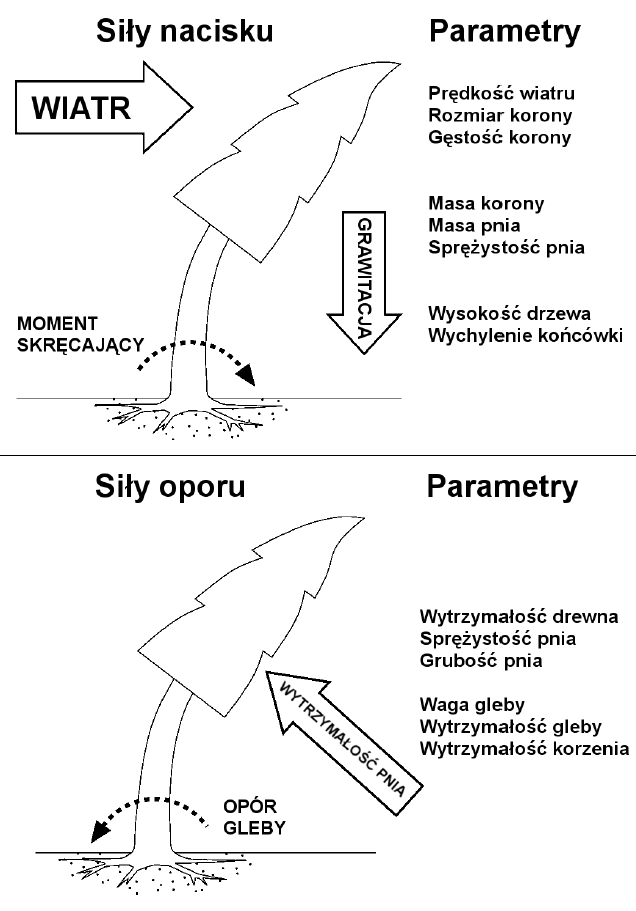
\includegraphics[scale=0.45]{HWIND1}
	\caption{Rozkład sił działających na drzewo dla modelu HWIND. Źródło: ~\cite{chm_mgza}.}
	\label{fig:HWIND1}
\end{figure} 

Rysunek ~\ref{fig:HWIND1} przedstawia siły działające na drzewo. Dokonany został podział na siły poziome i ~pionowe.
Pod naporem wiatru drzewo ugina się do momentu osiągnięcia punktu krytycznego, gdy siły nacisku (siła wiatru, siła grawitacji) zrównają się z ~siłami oporu (wytrzymałość pnia, wytrzymałość gleby wokół korzenia).

W celu wyznaczenia maksymalnego momentu skręcającego i ~granicznej prędkości wiatru przy której nastąpi zniszczenie drzewa, podzielone zostały one na 1~metrowe segmenty, dla których wyznaczone zostaną wartości sił.

Całkowita pozioma siła wiatru $F_w$ uzyskana zostaje poprzez sumowanie wartości siły wiatru obliczonej osobno dla każdego 1~metrowego segmentu ~\cite{chm_mgza}. Siła dla poszczególnego segmentu uzyskiwana jest ze wzoru:
$$ F_w(z) = \frac{1}{2}C_d  \rho v_h^2 A(z) $$ 
gdzie

\begin{description}
  \item[$C_d$] -- współczynnik tarcia
  \item[$\rho$ ]-- gęstość powietrza
  \item[$v_h$ ]-- prędkość pozioma dla danego segmentu
  \item[$A(z)$]-- przewidywana wielkość korony drzewa stawiająca opór wiatrowi
\end{description}

W celu uproszczenia obliczeń dokonana została aproksymacja powierzchni korony drzewa przez trójkąt równoramienny (świerk pospolity). Pole powierzchni pnia jest reprezentowane przez prostokąt. Model ten przedstawia rysunek \ref{fig:HWIND2}.

\begin{figure}[!h]
	\center
	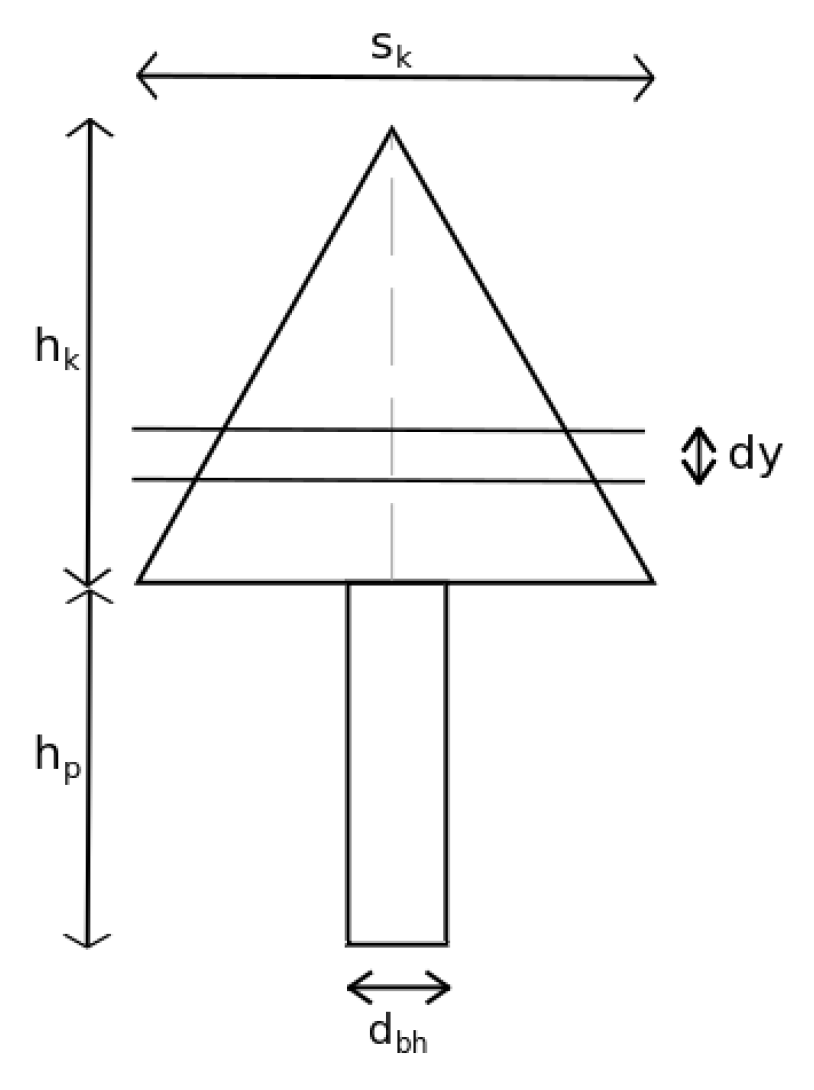
\includegraphics[scale=0.35]{HWIND2}
	\caption{Model powierzchni stawiającej opór wiatrowi. $s_k$ oznacza szerokość korony, $h_k$ -- wysokość korony, $h_p$ -- wysokość pnia, $d_{bh}$ -- średnicę pnia, $d_y$ -- wycinek powierzchni o wysokości 1m użyty przy w modelu HWIND. Źródło: ~\cite{chm_mgza}.}
	\label{fig:HWIND2}
\end{figure} 

W modelu należy uwzględnić fakt, iż pod wpływem wiatru powierzchnia korony ulega zmniejszeniu ~\cite{todo_jakies_zrodlo}. Redukcja powierzchni wynosi $20\%$ dla prędkości mniejszych od $11 \frac{m}{s}$, dla 
większych od $20\frac{m}{s}$ -- $60\%$. Dla wartości pomiędzy nimi współczynnik przepływu wiatru $S_t$ jest wyznaczany z następującego wzoru:
$$ S_t(z) = 0.044444v(z) - 0.28889$$
gdzie
\begin{description}
  \item[$v(z)$] -- prędkość wiatru na wysokości z
\end{description}

Powierzchnia $A(z)$ wyznaczana jest przez jej iloczyn ze współczynnikiem $S_t$.
\\

Siła grawitacji wyznaczana jest dla każdego segmentu drzewa, a następnie sumowana. Wyznaczana jest ze wzoru:
$$F_g(z) = m_c g$$
gdzie
\begin{description}
  \item[$m_c$] -- masa korony drzewa
  \item[$g$] -- przyspieszenie ziemskie
\end{description}


\clearpage
\input{Rankine}

\clearpage
\section{Opis implementacji}

\begin{figure}[!h]
	\center
	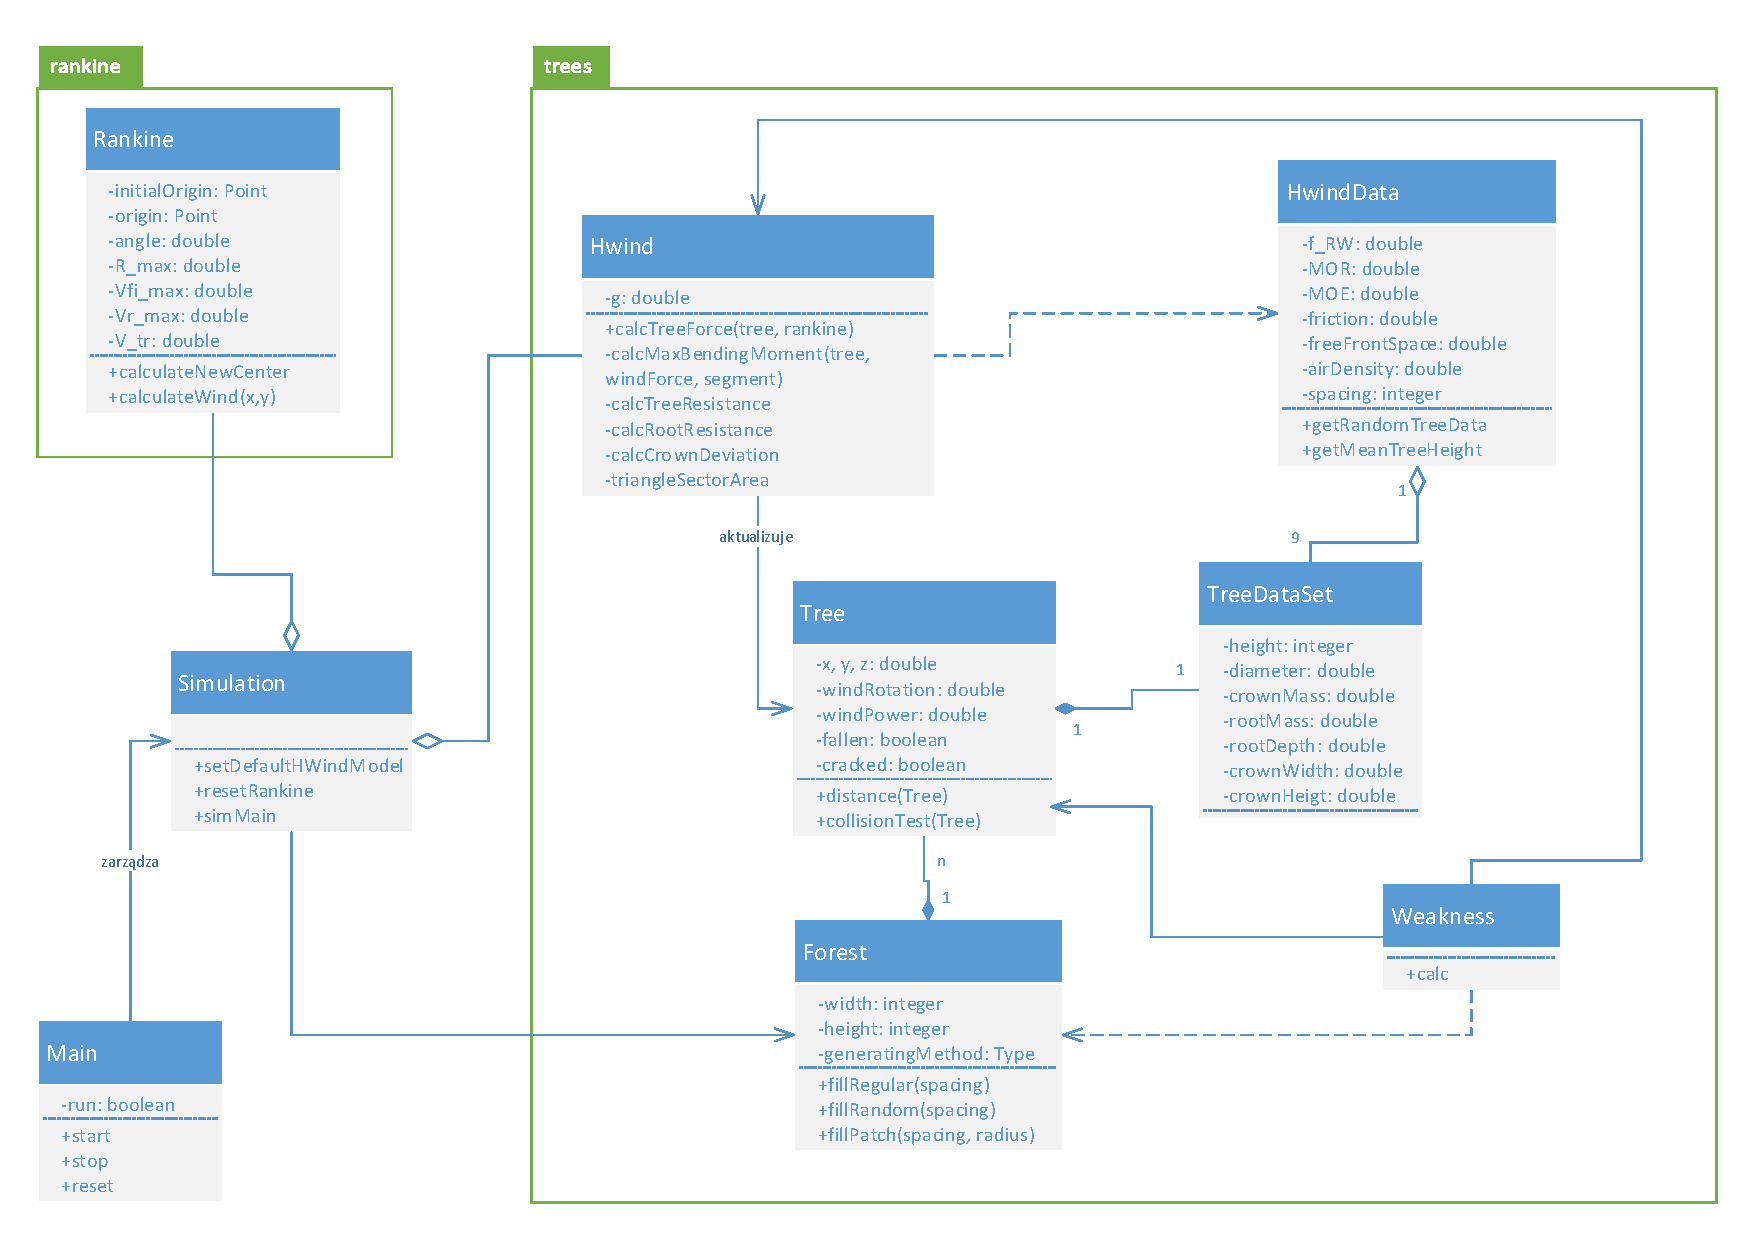
\includegraphics[scale=0.51]{uml}
	\caption{Diagram klas logiki aplikacji.}
	\label{fig:uml1}
\end{figure} 

Aplikacja została zaimplementowana w języku Java. 

Rysunek~\ref{fig:uml1} przedstawia zależności między klasami logiki aplikacji.

Głównymi klasami wpływającymi na przebieg symulacji są 
\begin{itemize}
\item Rankine (model wiru)
\item Hwind (model zniszczeń drzew)
\end{itemize}
Klasa Forest przechowuje informacje na temat parametrów lasu, takich jak jego wymiary, czy położenia drzew (przechowuje obiekty klasy Tree). Klasa Simulation stanowi element sterujący symulacji.
Klasy HwindData oraz TreeDataSet przechowują większość parametrów modelu zniszczeń drzew. Pierwsza posiada informacje średniej wysokości drzew w lesie, wartościach współczynnika tarcia oraz innych opisanych w charakterystyce modelu HWIND.
Druga z nich przechowuje informacje na temat konkretnego drzewa.

Klasa Weakness służy do wyznaczania wytrzymałości konkretnego drzewa w lesie na działanie siły wiatru (poprzez uwzględnienie jego sąsiedztwa).

Głównymi klasami które nas interesują z punktu widzenia użytkowników symulacji są klasy Tree i Forest. To one przechowują wynik symulacji.

 Rysunek~\ref{fig:uml2} przedstawia możliwe przypadki użycia. Aplikacja pozwala na przeprowadzenie symulacji zniszczeń, wraz z możliwością zmiany wartości jej parametrów. Działanie programu wizualizowane jest na bieżąco.

\begin{figure}[!h]
	\center
	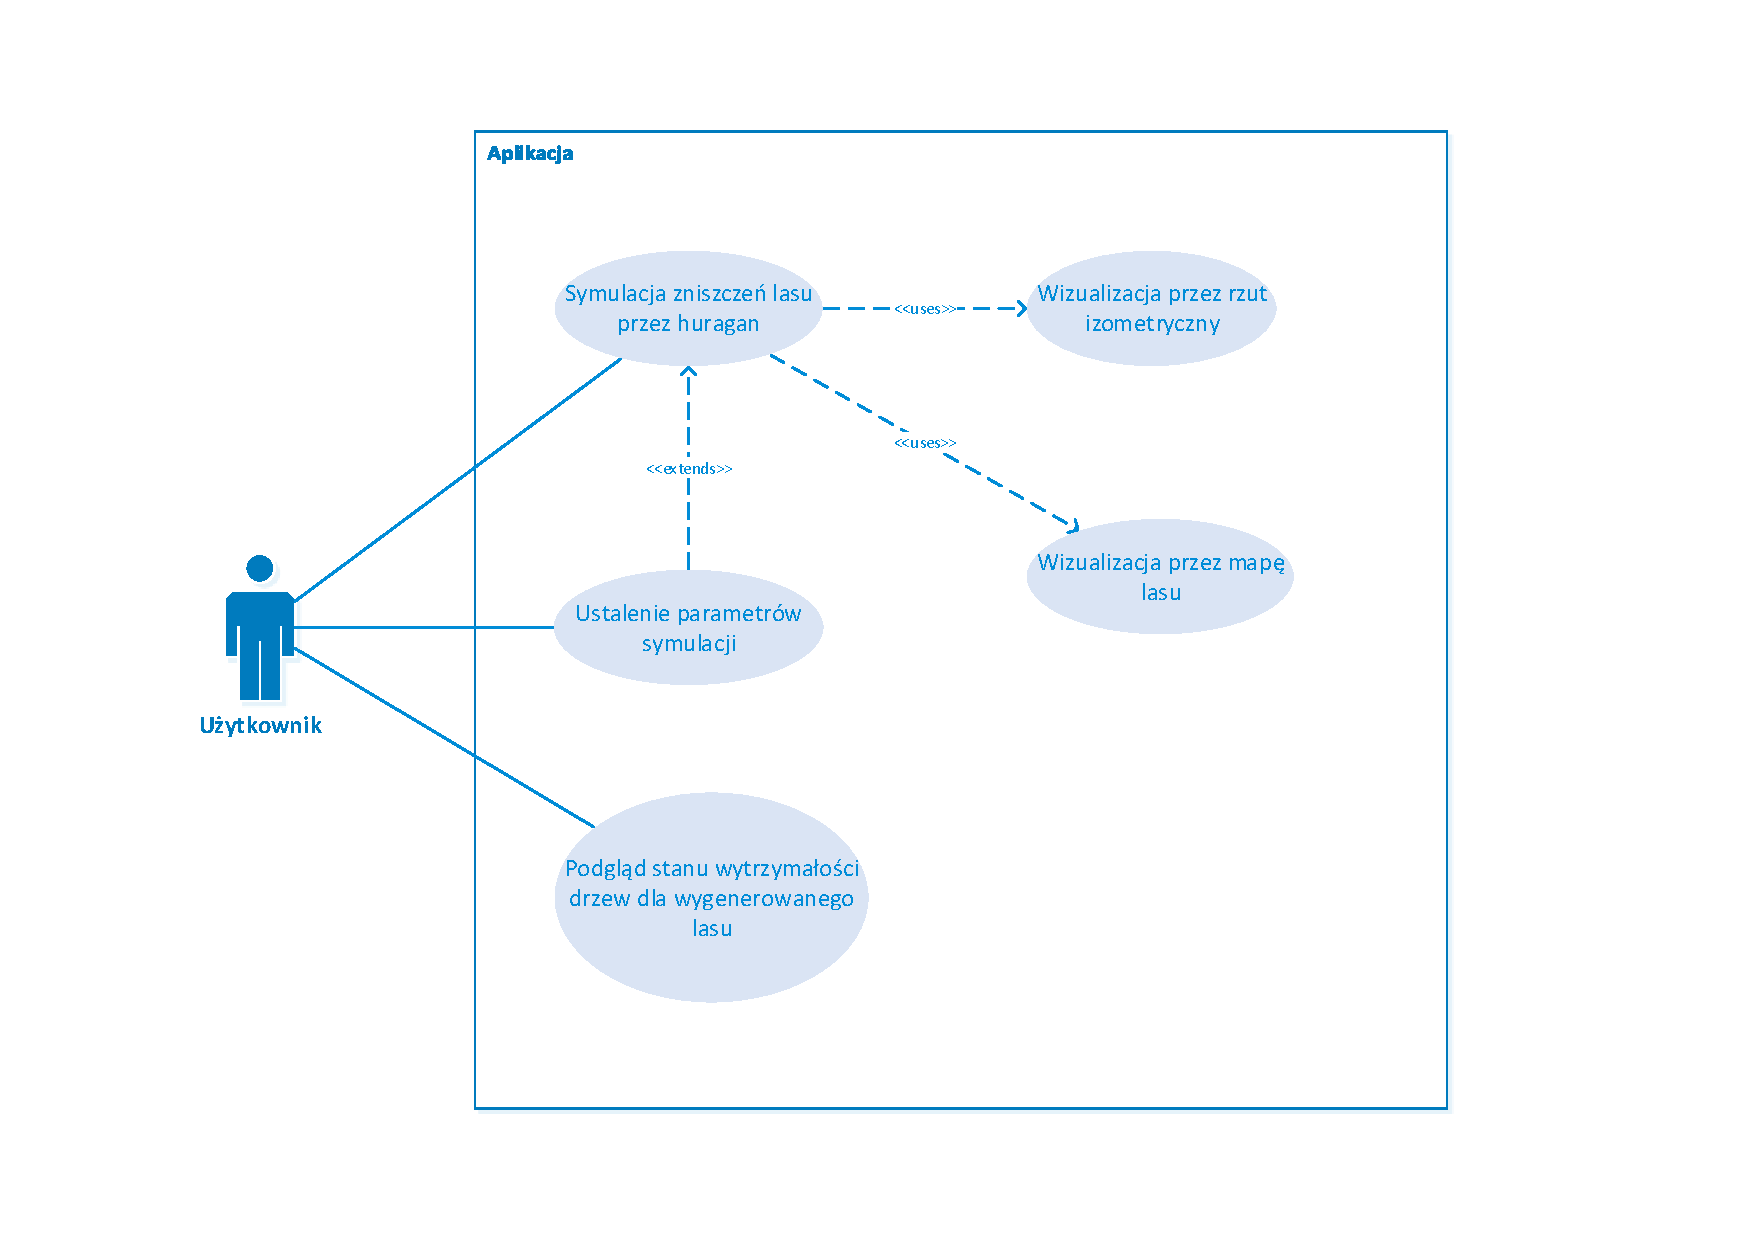
\includegraphics[scale=0.5]{uml_use_case}
	\caption{Diagram przypadków użycia.}
	\label{fig:uml2}
\end{figure} 

Zachowanie każdego drzewa zostało odzwierciedlone przez oddzielny wątek. Wykorzystując wzajemnie informacje o swym stanie, oraz obiekty klas modelu drzewa określają swój stan w danym momencie. Wykorzystanie koncepcji programowania agentowego pozwala na lepsze odzwierciedlenie rzeczywistej sytuacji, a co za tym idzie - uzyskania bardziej wiarygodnych wyników.







\clearpage
\section{Opis interfejsu}

\begin{figure}[!h]
	\center
	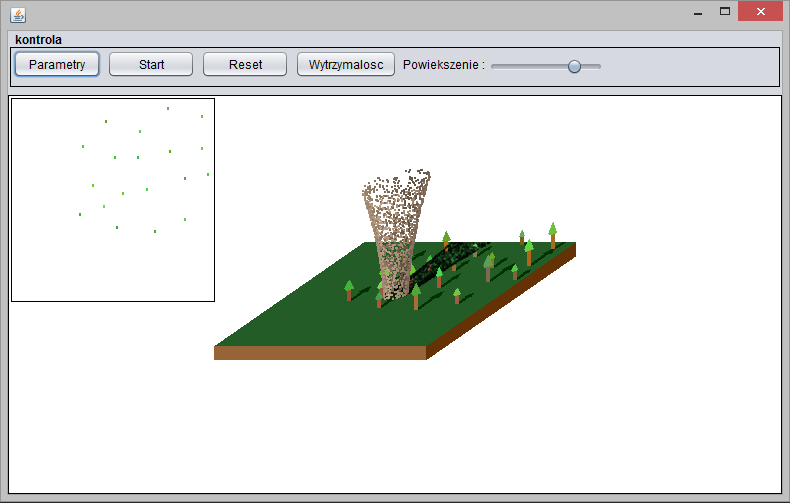
\includegraphics[scale=0.75]{gui_main}
	\caption{Główne okno programu.}
	\label{fig:gui_main}
\end{figure} 

Uruchamienie aplikacji symulacji powoduje wyświetlenie głównego okna programu (Rysunek~\ref{fig:gui_main}). W centralnej ramce ukazana jest wizualizacja zjawiska w rzucie izometrycznym. Ukazuje ona symboliczną strukturę lasu i położenie tornada. Drzewa nieuszkodzone mają pień koloru brązowego oraz zieloną koronę, drzewa złamane wizualizowane są w kolorze czerwonym, a drzewa przewrócone w kolorze niebieskim. W lewym górnym rogu ukazany jest rzut lasu z góry, który posiada taką samą konwencję kolorów jak wizualizacja 3D. Można na nim dokładniej zaobserwować kierunki działania wiatru tornada przy przewracaniu drzew.

Dodatkowo, przytrzymując przycisk \textbf{Wytrzymałość} możliwa jest wizualizacja potencjalnej wytrzymałości drzew wyliczana na podstawie otoczenia każdego z nich. Kolor niebieski oznacza najmniej wytrzymałe drzewo, czyli znajdujące się na skraju lasu i/lub nieposiadające bliskich sąsiadów. Im korona bardziej przechodzi w kolor czerwony, drzewo klasyfikowane jest jako bardziej wytrzymałe dzięki tłumieniu wiatru przez drzewa położone w najbliższym jego otoczeniu.

 Nad ramką wizualizacji znajduje się panel sterowania symulacją. Dotępne przyciski kontroli to:

\begin{itemize}
\item \textbf{Parametry} -- wyświetlenie okna ustawiania parametrów symulacji oraz właściwości modeli Rankine i HWind.
\item \textbf{Start/Stop} -- rozpoczęcie/zatrzymanie symulacji.
\item \textbf{Reset} -- przywrócenie wartości początkowych (ustawionych w oknie Parametry) symulacji, wygenerowanie nowego lasu.
\item \textbf{Wytrzymałość} -- przytrzymanie tego przycisku powoduje wyświetlenie informacji o wytrzymałości drzew w postaci kolorów.
\end{itemize}

Ponadto, istnieje możliwość zmiany skali wizualizacji przesuwając suwak z etykietą ,,Powiększenie'' na pożadaną pozycję.



\subsection{Okno parametrów symulacji}

Wygląd interfejsu manipulacji parametrami programu przedstawia rysunek~\ref{fig:gui_param}.

W ramce \textbf{Świat} możemy ustawić wymiary (szerokość i długość) siatki, na której zostanie wygenerowany las.

Ramka \textbf{Wir} pozwala na manipulację parametrami modelu wiru Rankine. Posiada następujące kontrolki:
\begin{itemize}
\item
\end{itemize}

\begin{figure}[!h]
	\center
	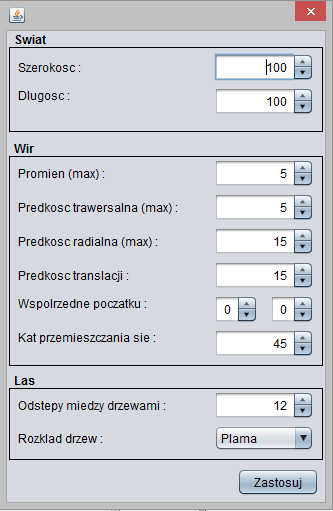
\includegraphics[scale=1]{gui_param}
	\caption{Okno ustawiania parametrów symulacji.}
	\label{fig:gui_param}
\end{figure} 

\clearpage
\section{Przykładowe wyniki symulacji}

Przeprowadzono przykładowe symulacje w celu zweryfikowania wyników oraz zwalidowania przyjętych modeli zjawisk fizycznych.
\subsection{Symulacja wąskiego tornada}

Parametry pierwszej symulacji przedstawia rysunek~\ref{fig:test1p}. Jest to dosyć wąskie tornado, przemierza prawie cały las pod kątek 45 stopni.

\begin{figure}[!h]
	\center
	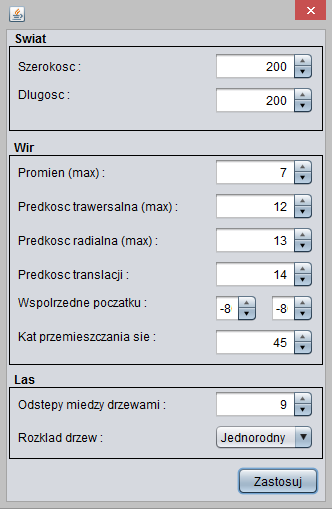
\includegraphics[scale=0.7]{test1p}
	\caption{Parametry pierwszej przykładowej symulacji.}
	\label{fig:test1p}
\end{figure} 

Wyniki symulacji zaprezentowane są na rysunku~\ref{fig:test1}. Jak widzimy, zgodnie z założeniami modelu tornado dokonało największych zniszczeń na obrzeżach lasu, gdzie wytrzymałości drzew są najmniejsze. Najlepiej przetrwały drzewa centralne, które otoczone są innymi drzewami.

\begin{figure}[!h]
	\center
	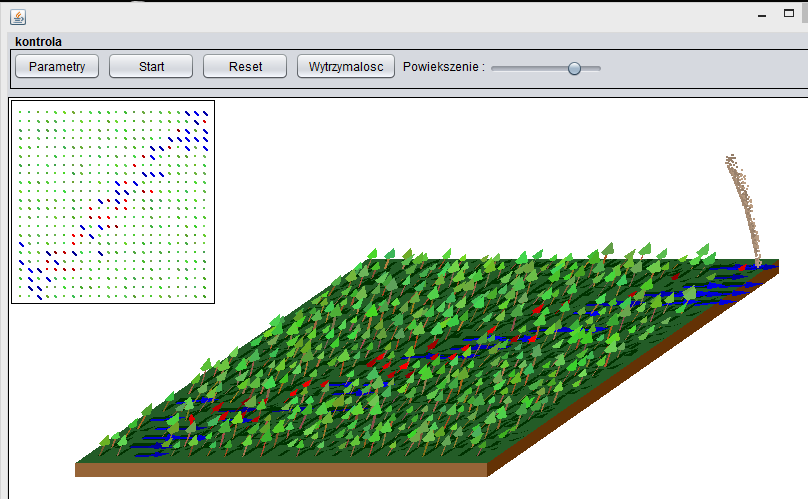
\includegraphics[scale=0.62]{test1}
	\caption{Wynik pierwszej przykładowej symulacji.}
	\label{fig:test1}
\end{figure} 

\subsection{Symulacja szerokiego tornada}

Parametry drugiej symulacji przedstawione są na rysunku~\ref{fig:test2p}. Jest to dosyć szersze tornado, o parametrach podobnych do pierwszego przykładu.

\begin{figure}[!h]
	\center
	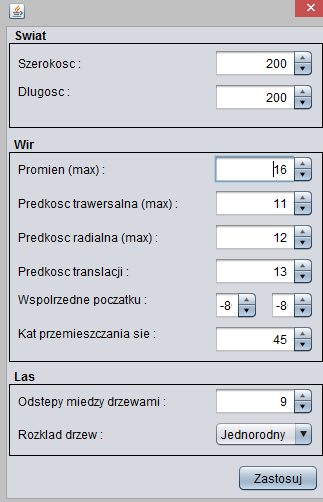
\includegraphics[scale=0.7]{test2p}
	\caption{Parametry drugiej przykładowej symulacji.}
	\label{fig:test2p}
\end{figure} 

Wyniki symulacji zaprezentowane są na rysunku~\ref{fig:test2}. Można zauważyć, iż tornado ma większy zasięg, jednak zwiększył się stosunek ilości drzew złamanych do ilości drzew przewróconych, co wskazuje na mniejszą siłę wiatru. Również w centrum tornada część drzew zostało nietkniętych, ponieważ w środku tornada panuje mniejszy wiatr. Tak jak w pierwszym przypadku można zaobserwować zmniejszoną wytrzymałość drzew na krańcach lasu.

\begin{figure}[!h]
	\center
	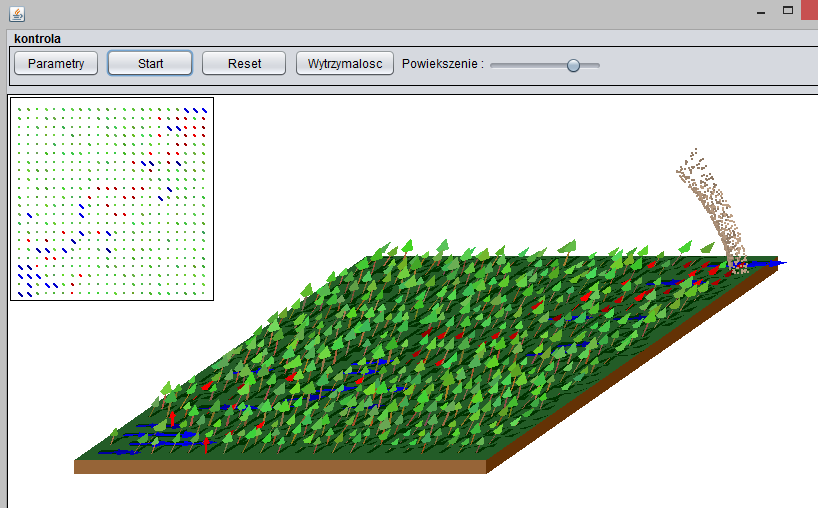
\includegraphics[scale=0.62]{test2}
	\caption{Wynik drugiej przykładowej symulacji.}
	\label{fig:test2}
\end{figure} 

\section{Walidacja}

Poddając model walidacji można się przekonać, czy wybrany model wiernie odwzorowuje rzeczywiste zjawiska fizyczne.
Zdjęcie~\ref{fig:walid1} przedstawia las po przejściu tornada w Hrabstwiw Rabun w stanie Georgia w Stanach Zjednoczonych. Można zauważyć, że tornado miało dużą szerokość, czym przypominało tornado z drugiej przykładowej symulacji. Widać także podobieństwo w skutkach -- oba tornada w przeważającej ilości tylko połamały drzewa, ponieważ nie posiadały wystarczającej siły aby je przewrócić.

\begin{figure}[!h]
	\center
	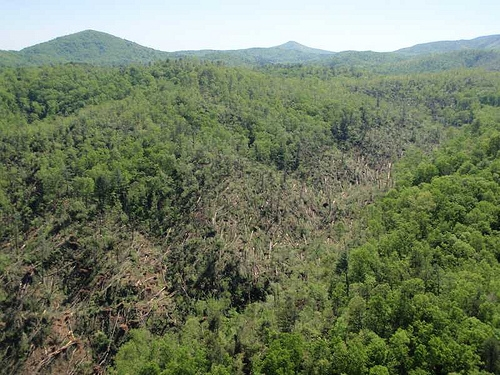
\includegraphics[scale=0.75]{walid1}
	\caption{Las po tornadzie w stanie Georgia.}
	\label{fig:walid1}
\end{figure} 

Zdjęcie~\ref{fig:walid2} ukazuje las w Parku Narodowmy Great Smoky Mountains na pograniczu stanów Karolina Północna i Tennessee w Stanach Zjednoczonych po przejściu tornada. Widać, że tornado miało większą siłę i było momentami stosunkowo wąskie. Tam, gdzie trzewa rosły rzadziej, tornado wyrządziło największe szkody. Na zewnątrz centrum tornada zostały wyrządzone większe szkody niż na trasie środka wiru. Można uznać, że dane te zgadzają się z przyjętym modelem.

\begin{figure}[!h]
	\center
	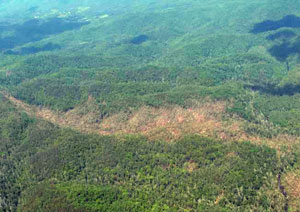
\includegraphics[scale=0.75]{walid2}
	\caption{Las po tornadzie w Parku Narodowmy Great Smoky Mountains.}
	\label{fig:walid2}
\end{figure} 

\clearpage
\section{Statystyki}

W celu prezentacji statystyk przeprowadzone zostały wielokrotne przebiegi symulacji.
Wyniki te pozwolą na określenie średniej wielkości zniszczeń i ekstremów.

Pierwszy zestaw symulacji został przeprowadzony dla parametrów:
\begin{itemize}
\item Wymiary: $200m x 200m$
\item Promień (max): $7m/s$
\item Prędkość trawersalna (max): $12m/s$
\item Prędkość radialna (max): $13m/s$
\item Prędkość translacji: $14m/s$
\item Punkt startowy: $(-8, -8)$
\item Kąt przemieszczania się wiru: $45$ stopni
\item Odstępy między drzewami: $9m$
\item Rozkład drzew: Jednorodny
\end{itemize}

Wyniki przedstawia tabela~\ref{tab:sym1}:

 \begin{table}[h!]
 \caption{Wyniki dla rozkładu jednorodnego.}
 \label{tab:sym1}
 \begin{center}
\begin{tabular} {|c|c|c|}
\hline
Wyrwane & Złamane & Początkowa liczba \\ \hline \hline
$28$ 	& $47$	&	$529$ \\ \hline
$37$ 	& $52$ 	&	$529$ \\ \hline
$34$ 	& $53$ 	&	$529$ \\ \hline
$46$ 	& $47$	&	$529$ \\ \hline
$42$ 	& $60$	&	$529$ \\ \hline
$34$ 	& $47$ 	&	$529$ \\ \hline
\end{tabular}
\end{center}
\end{table}


Analizując tabelę można stwierdzić, że stopień zniszczeń lasu dla zadanych parametrów nie jest duży. Średnia liczba wyrwanych drzew wyniosła około $37$ sztuk, w przypadku złamań: $51$. Największa liczba wyrwanych drzew jaka wystąpiła w przebiegach symulacji to $46$, najmniejsza: $28$. W przypadku złamań jest to odpowiednio $60$ i $47$.
Średnio zniszczonych zostało $16.64\%$ drzew.

Kolejny zestaw symulacji został przeprowadzony dla parametrów:
\begin{itemize}
\item Wymiary: $100m x 100m$
\item Promień (max): $7m/s$
\item Prędkość trawersalna (max): $12m/s$
\item Prędkość radialna (max): $13m/s$
\item Prędkość translacji: $14m/s$
\item Punkt startowy: $(-8, -8)$
\item Kąt przemieszczania się wiru: $45$ stopni
\item Rozkład drzew: Losowy
\end{itemize}

Wyniki przedstawia tabela~\ref{tab:sym2}:

 \begin{table}[h!]
 \caption{Wyniki dla rozkładu losowego.}
 \label{tab:sym2}
 \begin{center}
\begin{tabular} {|c|c|c|}
\hline
Wyrwane & Złamane & Początkowa liczba \\ \hline \hline
$30$ 	& $32$ 	&	$100$ \\ \hline
$23$ 	& $30$ 	&	$100$ \\ \hline
$33$ 	& $30$ 	&	$100$ \\ \hline
$27$ 	& $35$ 	&	$100$ \\ \hline
$24$ 	& $28$ 	&	$100$ \\ \hline
$26$ 	& $25$ 	&	$100$ \\ \hline
\end{tabular}
\end{center}
\end{table}


Stopień zniszczeń jest widocznie większy niż w poprzednich symulacjach. Spowodowane jest to głównie znacząco mniejszą liczbą drzew jak i nierównomiernym zagęszczeniem. Średnia liczba wyrwanych drzew wyniosła $27$, najmniejsza $23$, największa $33$. W przypadku złamanych drzew jest to odpowiednioi $30$, $25$, $35$.
Średnio zniszczonych zostało $57\%$ drzew.

Ostatni zestaw symulacji został przeprowadzony dla parametrów:
\begin{itemize}
\item Wymiary: $100m x 100m$
\item Promień (max): $7m/s$
\item Prędkość trawersalna (max): $12m/s$
\item Prędkość radialna (max): $13m/s$
\item Prędkość translacji: $14m/s$
\item Punkt startowy: $(-8, -8)$
\item Kąt przemieszczania się wiru: $45$ stopni
\item Rozkład drzew: Plama
\end{itemize}

Wyniki przedstawia tabela~\ref{tab:sym3}:

 \begin{table}[h!]
 \caption{Wyniki dla rozkładu typu `plama'.}
 \label{tab:sym3}
 \begin{center}
\begin{tabular} {|c|c|c|}
\hline
Wyrwane & Złamane & Początkowa liczba \\ \hline \hline
$26$ 	& $21$ 	&	$100$ \\ \hline
$14$ 	& $10$ 	&	$100$ \\ \hline
$19$ 	& $50$ 	&	$100$ \\ \hline
$11$ 	& $18$ 	&	$100$ \\ \hline
$24$ 	& $31$ 	&	$100$ \\ \hline
$7$ 	& $12$ 	&	$100$ \\ \hline
\end{tabular}
\end{center}
\end{table}

Wyniki tych przebiegów są bardzo zróżnicowane. Wynika to ze sposobu generowania lasu - niekiedy mogło się zdarzyć, iż wir nie przechodził bezpośrednio przez las, lecz po jego krawędzi, co wpłynęło znacząco na stopień zniszczeń. 
Średnia wyrwanych drzew: $17$, złamanych: $24$. Minimalna liczba wyrwanych to $7$ drzew, maksymalna $26$. Odpowiednio dla złamanych jest to $10$ i $50$.
Średnio zniszczonych zostało $41\%$ drzew.



\bibliography{books}{}
\bibliographystyle{plain}

\end{document}




